%% bare_conf.tex
%% V1.4b
%% 2015/08/26
%% by Michael Shell
%% See:
%% http://www.michaelshell.org/
%% for current contact information.
%%
%% This is a skeleton file demonstrating the use of IEEEtran.cls
%% (requires IEEEtran.cls version 1.8b or later) with an IEEE
%% conference paper.
%%
%% Support sites:
%% http://www.michaelshell.org/tex/ieeetran/
%% http://www.ctan.org/pkg/ieeetran
%% and
%% http://www.ieee.org/

%%*************************************************************************
%% Legal Notice:
%% This code is offered as-is without any warranty either expressed or
%% implied; without even the implied warranty of MERCHANTABILITY or
%% FITNESS FOR A PARTICULAR PURPOSE!
%% User assumes all risk.
%% In no event shall the IEEE or any contributor to this code be liable for
%% any damages or losses, including, but not limited to, incidental,
%% consequential, or any other damages, resulting from the use or misuse
%% of any information contained here.
%%
%% All comments are the opinions of their respective authors and are not
%% necessarily endorsed by the IEEE.
%%
%% This work is distributed under the LaTeX Project Public License (LPPL)
%% ( http://www.latex-project.org/ ) version 1.3, and may be freely used,
%% distributed and modified. A copy of the LPPL, version 1.3, is included
%% in the base LaTeX documentation of all distributions of LaTeX released
%% 2003/12/01 or later.
%% Retain all contribution notices and credits.
%% ** Modified files should be clearly indicated as such, including  **
%% ** renaming them and changing author support contact information. **
%%*************************************************************************


% *** Authors should verify (and, if needed, correct) their LaTeX system  ***
% *** with the testflow diagnostic prior to trusting their LaTeX platform ***
% *** with production work. The IEEE's font choices and paper sizes can   ***
% *** trigger bugs that do not appear when using other class files.       ***                          ***
% The testflow support page is at:
% http://www.michaelshell.org/tex/testflow/



\documentclass[conference]{IEEEtran}
%\documentclass[conference]{IEEEconf_allowlinks}
% Some Computer Society conferences also require the compsoc mode option,
% but others use the standard conference format.
%
% If IEEEtran.cls has not been installed into the LaTeX system files,
% manually specify the path to it like:
% \documentclass[conference]{../sty/IEEEtran}





% Some very useful LaTeX packages include:
% (uncomment the ones you want to load)


% *** MISC UTILITY PACKAGES ***
%
%\usepackage{ifpdf}
% Heiko Oberdiek's ifpdf.sty is very useful if you need conditional
% compilation based on whether the output is pdf or dvi.
% usage:
% \ifpdf
%   % pdf code
% \else
%   % dvi code
% \fi
% The latest version of ifpdf.sty can be obtained from:
% http://www.ctan.org/pkg/ifpdf
% Also, note that IEEEtran.cls V1.7 and later provides a builtin
% \ifCLASSINFOpdf conditional that works the same way.
% When switching from latex to pdflatex and vice-versa, the compiler may
% have to be run twice to clear warning/error messages.






% *** CITATION PACKAGES ***
%
\usepackage{cite}
\usepackage{listings} % FOR CODE BLOCK 
% cite.sty was written by Donald Arseneau
% V1.6 and later of IEEEtran pre-defines the format of the cite.sty package
% \cite{} output to follow that of the IEEE. Loading the cite package will
% result in citation numbers being automatically sorted and properly
% "compressed/ranged". e.g., [1], [9], [2], [7], [5], [6] without using
% cite.sty will become [1], [2], [5]--[7], [9] using cite.sty. cite.sty's
% \cite will automatically add leading space, if needed. Use cite.sty's
% noadjust option (cite.sty V3.8 and later) if you want to turn this off
% such as if a citation ever needs to be enclosed in parenthesis.
% cite.sty is already installed on most LaTeX systems. Be sure and use
% version 5.0 (2009-03-20) and later if using hyperref.sty.
% The latest version can be obtained at:
% http://www.ctan.org/pkg/cite
% The documentation is contained in the cite.sty file itself.




% NOTE: %% from wikibooks

\usepackage{color}

\definecolor{mygreen}{rgb}{0,0.6,0}
\definecolor{mygray}{rgb}{0.5,0.5,0.5}
\definecolor{mymauve}{rgb}{0.58,0,0.82}

\lstset{
  backgroundcolor=\color{white},   % choose the background color; you must add \usepackage{color} or \usepackage{xcolor}; should come as last argument
  basicstyle=\footnotesize,        % the size of the fonts that are used for the code
  breakatwhitespace=false,         % sets if automatic breaks should only happen at whitespace
  breaklines=true,                 % sets automatic line breaking
  captionpos=b,                    % sets the caption-position to bottom
  commentstyle=\color{mygreen},    % comment style
  deletekeywords={...},            % if you want to delete keywords from the given language
  escapeinside={\%*}{*)},          % if you want to add LaTeX within your code
  extendedchars=true,              % lets you use non-ASCII characters; for 8-bits encodings only, does not work with UTF-8
  firstnumber=1000,                % start line enumeration with line 1000
  frame=single,	                   % adds a frame around the code
  keepspaces=true,                 % keeps spaces in text, useful for keeping indentation of code (possibly needs columns=flexible)
  keywordstyle=\color{blue},       % keyword style
  language=Octave,                 % the language of the code
  morekeywords={*,...},            % if you want to add more keywords to the set
  numbers=left,                    % where to put the line-numbers; possible values are (none, left, right)
  numbersep=5pt,                   % how far the line-numbers are from the code
  numberstyle=\tiny\color{mygray}, % the style that is used for the line-numbers
  rulecolor=\color{black},         % if not set, the frame-color may be changed on line-breaks within not-black text (e.g. comments (green here))
  showspaces=false,                % show spaces everywhere adding particular underscores; it overrides 'showstringspaces'
  showstringspaces=false,          % underline spaces within strings only
  showtabs=false,                  % show tabs within strings adding particular underscores
  stepnumber=2,                    % the step between two line-numbers. If it's 1, each line will be numbered
  stringstyle=\color{mymauve},     % string literal style
  tabsize=2,	                   % sets default tabsize to 2 spaces
  title=\lstname                   % show the filename of files included with \lstinputlisting; also try caption instead of title
}
\usepackage{hyperref}


% *** GRAPHICS RELATED PACKAGES ***
%
\ifCLASSINFOpdf
   \usepackage[pdftex]{graphicx}
  % declare the path(s) where your graphic files are
  % \graphicspath{{../pdf/}{../jpeg/}}
  % and their extensions so you won't have to specify these with
  % every instance of \includegraphics
  % \DeclareGraphicsExtensions{.pdf,.jpeg,.png}
\else
  % or other class option (dvipsone, dvipdf, if not using dvips). graphicx
  % will default to the driver specified in the system graphics.cfg if no
  % driver is specified.
  % \usepackage[dvips]{graphicx}
  % declare the path(s) where your graphic files are
  % \graphicspath{{../eps/}}
  % and their extensions so you won't have to specify these with
  % every instance of \includegraphics
  % \DeclareGraphicsExtensions{.eps}
\fi
% graphicx was written by David Carlisle and Sebastian Rahtz. It is
% required if you want graphics, photos, etc. graphicx.sty is already
% installed on most LaTeX systems. The latest version and documentation
% can be obtained at:
% http://www.ctan.org/pkg/graphicx
% Another good source of documentation is "Using Imported Graphics in
% LaTeX2e" by Keith Reckdahl which can be found at:
% http://www.ctan.org/pkg/epslatex
%
% latex, and pdflatex in dvi mode, support graphics in encapsulated
% postscript (.eps) format. pdflatex in pdf mode supports graphics
% in .pdf, .jpeg, .png and .mps (metapost) formats. Users should ensure
% that all non-photo figures use a vector format (.eps, .pdf, .mps) and
% not a bitmapped formats (.jpeg, .png). The IEEE frowns on bitmapped formats
% which can result in "jaggedy"/blurry rendering of lines and letters as
% well as large increases in file sizes.
%
% You can find documentation about the pdfTeX application at:
% http://www.tug.org/applications/pdftex





% *** MATH PACKAGES ***
%
\usepackage{amsmath}
\usepackage{bm} % BOLD
% A popular package from the American Mathematical Society that provides
% many useful and powerful commands for dealing with mathematics.
%
% Note that the amsmath package sets \interdisplaylinepenalty to 10000
% thus preventing page breaks from occurring within multiline equations. Use:
%\interdisplaylinepenalty=2500
% after loading amsmath to restore such page breaks as IEEEtran.cls normally
% does. amsmath.sty is already installed on most LaTeX systems. The latest
% version and documentation can be obtained at:
% http://www.ctan.org/pkg/amsmath

\usepackage[capitalise]{cleveref}

% *** SPECIALIZED LIST PACKAGES ***
%
%\usepackage{algorithmic}
% algorithmic.sty was written by Peter Williams and Rogerio Brito.
% This package provides an algorithmic environment fo describing algorithms.
% You can use the algorithmic environment in-text or within a figure
% environment to provide for a floating algorithm. Do NOT use the algorithm
% floating environment provided by algorithm.sty (by the same authors) or
% algorithm2e.sty (by Christophe Fiorio) as the IEEE does not use dedicated
% algorithm float types and packages that provide these will not provide
% correct IEEE style captions. The latest version and documentation of
% algorithmic.sty can be obtained at:
% http://www.ctan.org/pkg/algorithms
% Also of interest may be the (relatively newer and more customizable)
% algorithmicx.sty package by Szasz Janos:
% http://www.ctan.org/pkg/algorithmicx



\usepackage{wrapfig,lipsum,booktabs} % PRETTIER TABLES
% *** ALIGNMENT PACKAGES ***
%
\usepackage{array}
% Frank Mittelbach's and David Carlisle's array.sty patches and improves
% the standard LaTeX2e array and tabular environments to provide better
% appearance and additional user controls. As the default LaTeX2e table
% generation code is lacking to the point of almost being broken with
% respect to the quality of the end results, all users are strongly
% advised to use an enhanced (at the very least that provided by array.sty)
% set of table tools. array.sty is already installed on most systems. The
% latest version and documentation can be obtained at:
% http://www.ctan.org/pkg/array


% IEEEtran contains the IEEEeqnarray family of commands that can be used to
% generate multiline equations as well as matrices, tables, etc., of high
% quality.




% *** SUBFIGURE PACKAGES ***
\ifCLASSOPTIONcompsoc
  \usepackage[caption=false,font=normalsize,labelfont=sf,textfont=sf]{subfig}
\else
  \usepackage[caption=false,font=footnotesize]{subfig}
\fi
% subfig.sty, written by Steven Douglas Cochran, is the modern replacement
% for subfigure.sty, the latter of which is no longer maintained and is
% incompatible with some LaTeX packages including fixltx2e. However,
% subfig.sty requires and automatically loads Axel Sommerfeldt's caption.sty
% which will override IEEEtran.cls' handling of captions and this will result
% in non-IEEE style figure/table captions. To prevent this problem, be sure
% and invoke subfig.sty's "caption=false" package option (available since
% subfig.sty version 1.3, 2005/06/28) as this is will preserve IEEEtran.cls
% handling of captions.
% Note that the Computer Society format requires a larger sans serif font
% than the serif footnote size font used in traditional IEEE formatting
% and thus the need to invoke different subfig.sty package options depending
% on whether compsoc mode has been enabled.
%
% The latest version and documentation of subfig.sty can be obtained at:
% http://www.ctan.org/pkg/subfig




% *** FLOAT PACKAGES ***
%
%\usepackage{fixltx2e}
% fixltx2e, the successor to the earlier fix2col.sty, was written by
% Frank Mittelbach and David Carlisle. This package corrects a few problems
% in the LaTeX2e kernel, the most notable of which is that in current
% LaTeX2e releases, the ordering of single and double column floats is not
% guaranteed to be preserved. Thus, an unpatched LaTeX2e can allow a
% single column figure to be placed prior to an earlier double column
% figure.
% Be aware that LaTeX2e kernels dated 2015 and later have fixltx2e.sty's
% corrections already built into the system in which case a warning will
% be issued if an attempt is made to load fixltx2e.sty as it is no longer
% needed.
% The latest version and documentation can be found at:
% http://www.ctan.org/pkg/fixltx2e


%\usepackage{stfloats}
% stfloats.sty was written by Sigitas Tolusis. This package gives LaTeX2e
% the ability to do double column floats at the bottom of the page as well
% as the top. (e.g., "\begin{figure*}[!b]" is not normally possible in
% LaTeX2e). It also provides a command:
%\fnbelowfloat
% to enable the placement of footnotes below bottom floats (the standard
% LaTeX2e kernel puts them above bottom floats). This is an invasive package
% which rewrites many portions of the LaTeX2e float routines. It may not work
% with other packages that modify the LaTeX2e float routines. The latest
% version and documentation can be obtained at:
% http://www.ctan.org/pkg/stfloats
% Do not use the stfloats baselinefloat ability as the IEEE does not allow
% \baselineskip to stretch. Authors submitting work to the IEEE should note
% that the IEEE rarely uses double column equations and that authors should try
% to avoid such use. Do not be tempted to use the cuted.sty or midfloat.sty
% packages (also by Sigitas Tolusis) as the IEEE does not format its papers in
% such ways.
% Do not attempt to use stfloats with fixltx2e as they are incompatible.
% Instead, use Morten Hogholm'a dblfloatfix which combines the features
% of both fixltx2e and stfloats:
%
% \usepackage{dblfloatfix}
% The latest version can be found at:
% http://www.ctan.org/pkg/dblfloatfix




% *** PDF, URL AND HYPERLINK PACKAGES ***
%
\usepackage{url}
% url.sty was written by Donald Arseneau. It provides better support for
% handling and breaking URLs. url.sty is already installed on most LaTeX
% systems. The latest version and documentation can be obtained at:
% http://www.ctan.org/pkg/url
% Basically, \url{my_url_here}.




% *** Do not adjust lengths that control margins, column widths, etc. ***
% *** Do not use packages that alter fonts (such as pslatex).         ***
% There should be no need to do such things with IEEEtran.cls V1.6 and later.
% (Unless specifically asked to do so by the journal or conference you plan
% to submit to, of course. )


% correct bad hyphenation here
\hyphenation{op-tical net-works semi-conduc-tor}


\begin{document}
%
% paper title
% Titles are generally capitalized except for words such as a, an, and, as,
% at, but, by, for, in, nor, of, on, or, the, to and up, which are usually
% not capitalized unless they are the first or last word of the title.
% Linebreaks \\ can be used within to get better formatting as desired.
% Do not put math or special symbols in the title.
\title{Inertia Wheel Inverted Pendulum}


% author names and affiliations
% use a multiple column layout for up to three different
% affiliations
\author{\IEEEauthorblockN{Ashwin Krishna}
\IEEEauthorblockA{Harvard University\\
Email: ashwin\_krishna@college.harvard.edu}
\and
\IEEEauthorblockN{Nao Ouyang}
\IEEEauthorblockA{Harvard University\\
Email: nouyang@g.harvard.edu}
}

% conference papers do not typically use \thanks and this command
% is locked out in conference mode. If really needed, such as for
% the acknowledgment of grants, issue a \IEEEoverridecommandlockouts
% after \documentclass

% for over three affiliations, or if they all won't fit within the width
% of the page, use this alternative format:
%
%\author{\IEEEauthorblockN{Michael Shell\IEEEauthorrefmark{1},
%Homer Simpson\IEEEauthorrefmark{2},
%James Kirk\IEEEauthorrefmark{3},
%Montgomery Scott\IEEEauthorrefmark{3} and
%Eldon Tyrell\IEEEauthorrefmark{4}}
%\IEEEauthorblockA{\IEEEauthorrefmark{1}School of Electrical and Computer Engineering\\
%Georgia Institute of Technology,
%Atlanta, Georgia 30332--0250\\ Email: see http://www.michaelshell.org/contact.html}
%\IEEEauthorblockA{\IEEEauthorrefmark{2}Twentieth Century Fox, Springfield, USA\\
%Email: homer@thesimpsons.com}
%\IEEEauthorblockA{\IEEEauthorrefmark{3}Starfleet Academy, San Francisco, California 96678-2391\\
%Telephone: (800) 555--1212, Fax: (888) 555--1212}
%\IEEEauthorblockA{\IEEEauthorrefmark{4}Tyrell Inc., 123 Replicant Street, Los Angeles, California 90210--4321}}




% use for special paper notices
%\IEEEspecialpapernotice{(Invited Paper)}

% make the title area
\maketitle

% As a general rule, do not put math, special symbols or citations
% in the abstract
\begin{abstract}
We explore the classic nonlinear controls problem, inverting a pendulum, using analyses learned in this class. Specifically, we look at using a flywheel to stabilize the pendulum. We build a physical system from scratch. In simulation, we derive the equations of motion and apply LQR and region of attraction analyses for our system. We additionally perform controllability analysis to the case where the full state may not be measurable, as happened in our physical system. In hardware, we successfully implement downward stabilization and swingup controls using both a PD controller an a bang-bang controller. We discuss the design decisions, design iterations, and present work toward implementing a controller for the inverted state.
\end{abstract}

% no keywords




% For peer review papers, you can put extra information on the cover
% page as needed:
% \ifCLASSOPTIONpeerreview
% \begin{center} \bfseries EDICS Category: 3-BBND \end{center}
% \fi
%
% For peerreview papers, this IEEEtran command inserts a page break and
% creates the second title. It will be ignored for other modes.
\IEEEpeerreviewmaketitle



\section{Introduction}
% no \IEEEPARstart
Pendulum is inherently unstable around upright fixed point.


%Example write-up:
% http://web.mit.edu/sjlevine/www/project_data/bicycle-planning/sjlevine_final_report.pdf
% ttps://en.wikipedia.org/wiki/Nonlinear_system

\hfill mds

\hfill May 22, 2019

%\subsection{Todo}
%Control authority analysis -- max torque output as function of motor and flywheel (torque constraints)
%Compare to mglsin theta -- what is the maximum deviation angle we can recover from

\section{Hardware Methods}

First, motor with encoder, and small flywheel.
Insert picture of the three iterations.

(Final motor was a drill motor, available for ~\$25 at harbor freight)

\subsection{Theory to Reality}

Below, we will explain the LQR theory. However, in reality we relied on PD
control. The reasons for this are:

\begin{itemize}
    \item Limited torque output
    \item Lack of motor encoder
    \item Lack of current control -- our software controller outputs torque, but
    we do not command torque directly, and needed to write an inner PID loop  (I
    can fill this in)
\end{itemize}


\textbf{To calculate the state variables}, 
We have discrete digital values from the quadrature encoder on the shaft, which
was a high quality one (1025 counts).

We furthermore use a naive method to estimate angular velocities from the
encoder counts: measure time elapsed and the change in angle, divide, set as our
thetadot.

(Non constant time frame)

\subsection{Swingup with Bang-Bang Control}

\subsection{Inversion with PD Control}

We used a simple control with two k values: one for theta, and one for thetadot.
This is equivalent to a PD controller.

\subsection{Results}

Insert a table here! Our excellent results.

And link to the videos.


\section{Simulation Analysis}

\subsection{Equations of Motion}

To derive the equations of motion (EOM), we use the Lagrangian method. Let $L$
equal to the kinetic energy plus the potential energy of the system.


\begin{align}
    L = KE - PE
\end{align}

By Lagrange's method,

\begin{align}
    \frac{d}{dt} (\frac{\partial{L}}{\partial \dot{q}_i}) -
    \frac{\partial{L}}{\partial q_i}  &= \sum_{i=0}^{n} F_i
\end{align}

for $i = 1,2,3 ... n $ forces.

Thus, we need to write out the KE, the PE, the derivative of L with respective
to each state $q$, the derivative of L with respect to the (time) derivative of
each state $q$, and then the time derivative of that last term.

Let us first consider the unaltered case, from the problem set, where here we
will derive the equations of motion by hand but otherwise simply explain the
derivation in detail. Later, we will consider a system that more closely matches
our real-life system. We will not be able to compare the model with reality,
since we were unable to implement the full state measurement so LQR cannot
apply. Instead, we show another example as applied to a modified system where
the reaction wheel pendulum is put on an (unpowered) cart.


\noindent 1) \textbf{Write the KE of the system}. We can decompose this into the translational and
rotational components.

First, let us consider (abstractly) the translational KE of a point mass $m$ rotating
around the origin on a massless string of length $l$. $\theta$ is defined as
angle from the downward vertical point, increasing counterclockwise  (diagram not provided).
The position of the point mass is $x = l cos \theta$ and $y = l sin \theta$.
KE is $\frac{1}{2} m \cdot q^2$, where q is the position.

% http://underactuated.csail.mit.edu/underactuated.html?chapter=multibody
\begin{align}
    KE_x &= 0.5 m (l \cdot \frac{d}{dt} \sin \theta)^2 = \frac{1}{2} m (l \dot\theta \cos \theta)^2 \\
    KE_y &= 0.5 m (l \cdot \frac{d}{dt} \cos \theta)^2  = \frac{1}{2} m (- l \dot\theta \sin\theta)^2 \\
    KE &= KE_x + KE_y = \frac{1}{2} m l^2 \dot \theta^2 (\cos^2 \theta + \sin^2 \theta) \\
       &= \frac{1}{2} m l^2 \dot\theta^2 \\
\end{align}

where on the last step we used the trig identity $\cos^2 + sin^2 = 1$.

Now applying this to the stick and flywheel components of our system, we
calculate 1) the stick around the origin 2) the flywheel around the origin. Note
that the KE of the stick acts at $l_1$, the center-of-mass of the stick, not
$l_2$.

\begin{align}
    KE_{\text{translational}} &= \frac{1}{2} m_1 (l_1 \dot\theta_1)^2 + \frac{1}{2} m_2 (l_2 \dot\theta_1)^2\\
\end{align}

Additionally we have the inertial component of KE since we have angular
velocities here and our stick has mass and our previous point mass is instead a rotating
flywheel. The general formula is $KE = \frac{1}{2} I_2 \dot\theta^2$.
Noting that angular velocities "add", and applying this to each component of our
system; we calculate 1) inertial KE of the stick 2) inertial KE of the flywheel.
\begin{align}
    KE_{\text{inertial}} &= \frac{1}{2} I_1 \dot\theta_1^2 + \frac{1}{2}
    I_2 (\dot\theta_1 + \dot\theta_2)^2
\end{align}

The total KE of the system is the sum of the above.

\noindent 2) \textbf{Write the PE of the system}. This is more straightforward. Gravitationally
speaking, (and with a bit of geometry - note that our theta is defined from
vertical and increasing counterclockwise)
\begin{align}
    PE &= m_1 g (- l_1 \cos\theta_1) + m_2 g (- l_2 \cos\theta_1)
\end{align}

\noindent 3) Now we have the Lagrangian $L = KE - PE$ and must take the partial of the Lagrangian with
respect to each state variable, in our case $\theta_1$ and $\theta_2$.

Using sympy (note: we left the sympy ordering intact, so the terms are a
bit weird), we calculate
\begin{align}
    \frac{\partial L}{\partial q} &=
    \begin{bmatrix}
        -g l_1 m_1 \sin(\theta_1) - g l_2 m_2 \sin(\theta_1) \\
        0
    \end{bmatrix}
    \label{eq:partialq}
\end{align}

\noindent 4) As an intermediate step, we calculate the
\begin{align}
    \frac{\partial L}{\partial \dot q} &=
    \begin{bmatrix}
        I_1 \dot\theta_1 + I_2 (\dot\theta_1 + \dot\theta_2) +
            l_1^2 m_1 \dot\theta_1 + l_2^2 m_2 \dot \theta_1 \\
            I_2 (\dot \theta_1 + \dot\theta_2)
    \end{bmatrix}
    \label{eq:partialqdot}
\end{align}

\noindent 5) Finally, we calculate the time derivative of the previous term
\begin{align}
    \frac{d}{dt} \frac{\partial L}{\partial \dot q_i} &=
    \begin{bmatrix}
    I_2 \ddot\theta_2 + \ddot\theta_1 ( I_1 +  I_2 +  m_1 l_1^2 + m_2 l_2^2) \\
    I_2 \ddot\theta_1 + I_2 \ddot\theta_2
    \end{bmatrix}
    \label{eq:ddt}
\end{align}

\noindent 6) We set the equation equal, on the right hand side, to our input torque $\tau$.

We may then directly ask sympy to solve for $\ddot q$

\begin{align}
    \ddot \theta_1 &= -g \frac{ (m_1 l_1 + m_2 l_2) \sin(\theta_1)}
        {I_1 + m_1 l_1^2 + m_2 l_2^2} \\
    \ddot \theta_2 &= g \frac{ (m_1 l_1 + m_2 l_2) \sin(\theta_1) }
        {I_1 + m_1 l_1^2 + m_2 l_2^2}
\end{align}

More neatly, we can go directly from \cref{eq:ddt} and
\cref{eq:partialq} to the "manipulator equations" as per the class textbook.
Specifically, we put \cref{eq:ddt} on the left hand side, factoring out
$\ddot \theta_1$ and $\ddot \theta_2$; then on the right hand side we put
\cref{eq:partialq}, factoring out $\dot \theta_1$ and $\dot \theta_2$ as well as
adding in our input torque $\tau$.

That is, we rewrite in form

\begin{equation}
\bm{M(q) \ddot q + C (q, \dot q) \dot q = \tau_g (q) + B u}
\end{equation}

Doing so, we then get as given to us in the homework
(yay it matches!)

\begin{align}
    \begin{bmatrix}
        m_1 l_1 ^2 + m_2 l_2^2 + I_1 + I_2 & I_2 \\
        I_2 & I_2
    \end{bmatrix}
    \begin{bmatrix}
        \ddot \theta_1 \\
        \ddot \theta_2
    \end{bmatrix}
    + 0
    &= \nonumber \\
    \begin{bmatrix}
        - (m_1 l_1 + m_2 l_2) g \sin\theta_1 \\
        0
    \end{bmatrix}
     +
     \begin{bmatrix}
         0 \\
         1
     \end{bmatrix}
     \tau
\end{align}


%\subsubsection{Motor vs Gravity}

%Tangentially, ideally our output torque is enough to fight gravity and
%essentially "hold" the pendulum floating in space at any angle, and the maximum
%torque is at horizontal ( $\theta_1 = \pi/2$ ).

%\begin{align}
    %\tau_{motor, max} &= 270 \; \text{Nm} \\
%\tau_{gravity, max} &= m g l sin\theta \\
%\tau_{gravity, max} &= m_{system} \cdot 9.8 \cdot 0.021 \cdot sin(\pi/2)\\
%\tau_{gravity, max} &= (.546 + .45 + .115/2 ) \cdot 9.8 \cdot 0.021 \cdot 1\\
%\tau_{gravity, max} &\approx .21 \; \text{Nm}
%\end{align}

%Where for back-of-envelope purposes we're approximating torque contribution of
%the stick.

%Here we easily see that our output torque does not approach this. A more
%useful analysis is to observe whether
%conservation of energy, we can conclude that for a closed system,

%\subsection{Find the Fixed Points}

%To find the fixed points of the system, we calculate $\dot q s.t. f(\dot q) = 0$

\subsection{Linearization Around Fixed Point}

We can further use sympy to linearize our fixed points.

Focusing on the upright case, we can use the approximation

\begin{align}
    \sin\theta \approx \pi - \theta \text{ for } \theta \approx \pi
\end{align}

For the downward case, we can similarly use the approximation

\begin{align}
    \sin\theta \approx \theta \text{ for } \theta \approx 0
\end{align}

% https://en.wikipedia.org/wiki/Nonlinear_system#Pendula
% TODO: push sympy code
After plugging in to sympy, we get 

\begin{lstlisting}[language=Python, frame=single]
t1ddot= -g*(l1*m1 + l2*m2)*sin(t1)/(I1 + l1**2*m1 + l2**2*m2)
t2ddot= g*(l1*m1 + l2*m2)*sin(t1)/(I1 + l1**2*m1 + l2**2*m2)
\end{lstlisting}

Or written in Latex,
\begin{align}
    \ddot \theta_1 &= -g \frac{(m_1 l_1 + m_2 l_2) \sin(\theta_1) } 
    {I_1 + m_1 l_1^2 + m_2 l_2^2)} \\
    \ddot \theta_2 &= g \frac{(m_1 l_1 + m_2 l_2) \sin(\theta_1) } 
    {I_1 + m_1 l_1^2 + m_2 l_2^2)}
\end{align}


This can be rewritten to be the same result as in the homework, where we
substitute in the approximation around $\theta = \pi$

\begin{align}
    \begin{bmatrix}
        \dot\theta_1 \\
        \dot\theta_2 \\
        \ddot\theta_1 \\
        \ddot\theta_2
    \end{bmatrix}
    =&
    \begin{bmatrix}
        0 & 0 & 1 & 0 \\
        0 & 0 & 0 & 1 \\
        \frac{(m_1 l_1 + m_2 l_2) g}{(m_1 l_1^2 + m_2 l_2^2 + I_1)} & 0 & 0 & 0 \\
        - \frac{(m_1 l_1 + m_2 l_2) g}{(m_1 l_1^2 + m_2 l_2^2 + I_1)}  & 0 & 0 & 0
    \end{bmatrix}
    \begin{bmatrix}
        \theta_1 - 180 \\
        \theta_2 \\
        \dot{\theta_1} \\
        \dot{\theta_2}
    \end{bmatrix} \nonumber \\
    &+
    \begin{bmatrix}
        0 \\
        0 \\
        \frac{-1}{(m_1 l_1^2 + m_2 l_2^2 + I_1)} \\
        \frac{1}{I_2} + \frac{1}{(m_1 l_1^2 + m_2 l_2^2 + I_1)}
    \end{bmatrix}
    \begin{bmatrix}
        \tau \\
    \end{bmatrix}
\end{align}

\subsubsection{A and B}

If we plug in the measurements from our physical system as in
\cref{tbl:systemparameters}, we get the following A and B matrices (rounded).

\begin{align}
    A &= 
    \begin{bmatrix}
        0 & 0 & 1 & 0 \\
        0 & 0 & 0 & 1 \\
        312 & 0 & 0 & 0 \\
        -312  & 0 & 0 & 0
    \end{bmatrix} \\
    B &=  
    \begin{bmatrix}
        0 \\
        0 \\
        -1395\\
        1901
    \end{bmatrix}
\end{align}
%originally A is  5 -5. and B is -0.1 11

Note: We treat the stick mass as negligible compared the motor, which is
modelled as a point mass at distance $l_2$; thus we set $l_1$ equal to $l_2$,
and $m_1$ = $m_{motor}$.

\begin{figure}[!t]
    \centering
    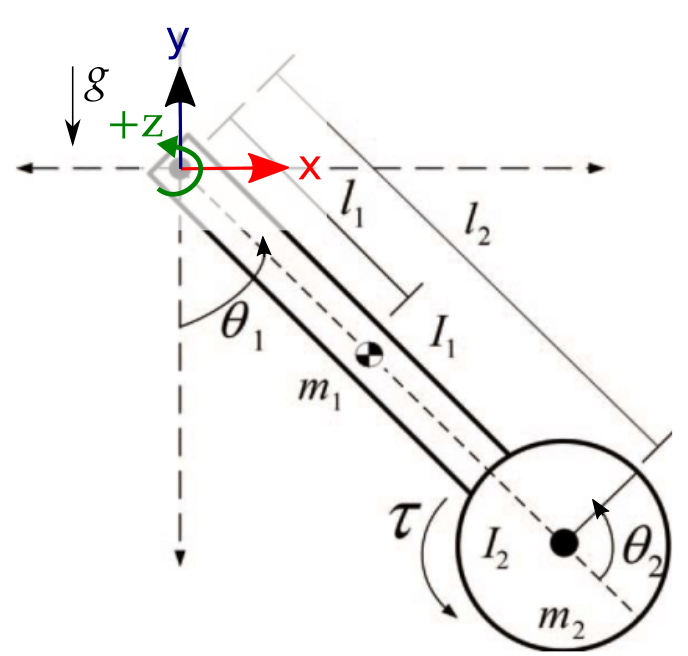
\includegraphics[width=0.5\linewidth]{images/freebody.png}
    \caption{Free body diagram}
    \label{}
\end{figure}

\subsection{Constants}

\begin{table}[!t]
    \renewcommand{\arraystretch}{1.5}
    \caption{System Constants}
    \label{tbl:systemparameters}
    \centering
    \begin{tabular}{|c|c|}
        \hline
        Property & Measurement \\
        \hline
        $m_{stick} = m_1$ & 115 g \\
        $m_{flywheel}$ & 546 g\\
        $m_{motor}$ & 450 g \\ % TODO: estimated
        $l_{stick} = l_2$ & 21 cm \\
        $r_{flywheel}$ & 8.5 cm \\ % TODO: estimated
        \hline
    \end{tabular}
\end{table}

\subsection{Applying LQR}

Now that we have $A$ and $B$, the matrices for our linearized dynamics of form
$f(x) = Ax + Bu$, we supply our Q and R cost functions and apply lqr. We care a
lot about the $\theta_1$, some about the $\dot\theta_1$, a bit about
$\dot\theta_2$, and not at all about $\theta_2$.  We also put a cost on the
input using $\textbf{R}$(here we closely follow the
assignment, since it turns out we will not be able to apply LQR to our physical
system).
%% ---------------------------------------------------------------------------
%% TODO ! change the inertia matrix and redo these numbers
%% ---------------------------------------------------------------------------
%% ---------------------------------------------------------------------------
\begin{align}
    Q &=
    \begin{bmatrix}
        10 & 0 & 0 & 0 \\
        0 & 1 & 0 & 0 \\
        0 & 0 & 0 & 0 \\
        0 & 0 & 0 & 0.1
    \end{bmatrix}\\
    R &= \begin{bmatrix} 0.1 \end{bmatrix}
\end{align}

Using the LQR function built into Drake, we get (rounded)

\begin{align}
    K &=
    \begin{bmatrix}
        -35 & 0 & -5 & -1 \\
    \end{bmatrix}\\
    S &=
    \begin{bmatrix}
        12 & 0 & 1  & 0. \\
        0 & 0 & 0 & 0 \\
        1 & 0 & 0. & 0. \\
        0. & 0 & 3 & 0.
    \end{bmatrix}
\end{align}

where K is our control matrix, operating on each of the four states ($q =
\theta_1, \theta_2, \dot \theta_1, \dot \theta_2$); and S is the solution of the
Ricatti equation.

% TODO: explore this S matrix further!!!
% Define what is the associated Ricatti equation

\subsection{Region of Attraction via Lyapunov}

We will briefly cover the region of attraction (RoA) analysis, which is covered
in the problem set already. For an LQR controller, which uses a linearization of
underlying nonlinear dynamics, this analysis tells us the region for which the
linearization is valid (where our LQR control can be used). 

Specifically, we will use Lyapunov analysis. Lyapunov analysis is a relaxed
optimization guarantee -- instead of guaranteeing an controller optimal for all
states will be found, we instead guarantee a controller will be able to
accomplish a given state. 

With the LQR controller, which operates as a constant matrix times the 
state error (from the desired fixed point)

\begin{align}
    u &= - K(x_{\text{measured}} - x_{\text{fixed point}})
\end{align}

We denote the error as $\bar x = x - x_{fp}$. For our Lyapunov function, we can use the cost-to-go of the LQR solution 

\begin{align}
    V_{\text{cost-to-go}} &= \bar x^T S \bar x
\end{align}

% TODO definte lyapunov function
where $S$ is as return to us by the Drake LQR solver. This S is the solution to
the Ricatti equation (a randomly fancy name for a first order quadratic
differential equation); in steady-state, this becomes an algebriac Ricatti
equation.

Note that in performing this analysis we picked a single known
reasonble Lyapunov function. Other functions are possible, which would give
slightly different regions of attraction for the same LQR controller.

% TODO: go more into this?

The value of this function, for a given state, can then be used to bound where
our linear controls will work. In our controller, we simply check the value of
$V$ for the state we are in and compare it to this bound. If we are within the
region of attraction, we use the LQR controller. Otherwise, we use the 
swing-up controller described in the following section.

\subsection{Energy-based Controller for Swingup}

% http://underactuated.csail.mit.edu/underactuated.html?chapter=acrobot
The idea behind the energy-based swingup controller is straightforward: we add
torque in the direction that the magnitude of $\theta_1$ is increasing in. We
care to increase $\theta_1$. However, we cannot directly control $\theta_1$, but
instead apply torque to control $\theta_2$. (In jargon, this is called
"non-collocated input").

For the simple pendulum, we observed 

\begin{align}
    \dot E &= u \dot \theta
\end{align}

For our system, we rederive $\dot E$ accounting for the fact that our input is
now non-collocated.

We actually desire $\dot E$ to be zero, since our $E$ will be at steady-state,
thus our energy error is directly $\dot E$. We then derive what u must be to
drive this to zero.

% TODO

In the end, in the actual sytem, a bang-bang controller was sufficient.
Additionally, as the derivation is already covered in the homework, we will not
repeat it here.

\subsection{Controllability}

This is again covered in the homework and will not be derived here.

The existence of multiple examples online would show that this system is
generally theoretically controllable, even given torque limits. 

In our case, we can also more directly consider a quick-and-dirty calcuation:
what is maximum torque produced by gravity, compared to the maximum torque our
motor can generate? Additionally, in reality the flywheel will also saturate at
some max speed of the motor, past which back EMF will limit the speed of the
flywheel. This strongly impacts the difficulty of controlling our system. 

This analyses is omitted, as the results didn't quite match reality, and likely
would need to be tailored further for the non-idealities of our physical system.

% TODO

\subsection{Is it Underactuated?}

When talking to friends about this, one of the first questions asked was
invariable "is that really an underactuated system?" especially since we do not
care about $\theta_2$.

By the definition in the textbook, 
    A control system described by equation 1 is underactuated in state (q,q˙) at
    time t if it is not able to command an arbitrary instantaneous acceleration
    in q.
With the particular caveat that the same system could be technically be fully or underactuated at different moments in time.

\section{LQR for "System on Wheels"}

%https://ocw.mit.edu/courses/mechanical-engineering/2-003sc-engineering-dynamics-fall-2011/lagrange-equations/MIT2_003SCF11_rec8notes1.pdf

For a detour (in order to demonstrate understanding of the problem set material)
we imagine sticking the whole thing on wheels and redo the same analysis,
although for sanity we run the calculations through sympy instead of by hand.
\cite{JS-aruco}


%\subsection{Controllability}

%We begin by analyzing the controllability of the system. At an intuitive level,
%we see that we've added a state (the x position of the cart) without adding any
%control inputs (we can still only control the flywheel directly). We might
%expect that we can still stabilize the system, but cannot control the cart
%position while keeping the pendulum upright (at least with LQR feedback).

%To check our intuition, we check the rank of the controllability matrix, defined as



%RS-550S-18V
%https://www.harborfreight.com/18-volt-cordless-38-drilldriver-with-keyless-chuck-68239.html
%https://grabcad.com/library/rs-550s-18v-harbor-freight-900rpm-18v-cordless-drill-motor-and-gearbox-1#!


\subsubsection{Equations of Motion}

\subsubsection{Linearization}
% An example of a floating figure using the graphicx package.
% Note that \label must occur AFTER (or within) \caption.
% For figures, \caption should occur after the \includegraphics.
% Note that IEEEtran v1.7 and later has special internal code that
% is designed to preserve the operation of \label within \caption
% even when the captionsoff option is in effect. However, because
% of issues like this, it may be the safest practice to put all your
% \label just after \caption rather than within \caption{}.
%
% Reminder: the "draftcls" or "draftclsnofoot", not "draft", class
% option should be used if it is desired that the figures are to be
% displayed while in draft mode.
%
%\begin{figure}[!t]
%\centering
%\includegraphics[width=2.5in]{myfigure}
% where an .eps filename suffix will be assumed under latex,
% and a .pdf suffix will be assumed for pdflatex; or what has been declared
% via \DeclareGraphicsExtensions.
%\caption{Simulation results for the network.}
%\label{fig_sim}
%\end{figure}

% Note that the IEEE typically puts floats only at the top, even when this
% results in a large percentage of a column being occupied by floats.


% An example of a double column floating figure using two subfigures.
% (The subfig.sty package must be loaded for this to work.)
% The subfigure \label commands are set within each subfloat command,
% and the \label for the overall figure must come after \caption.
% \hfil is used as a separator to get equal spacing.
% Watch out that the combined width of all the subfigures on a
% line do not exceed the text width or a line break will occur.
%
%\begin{figure*}[!t]
%\centering
%\subfloat[Case I]{\includegraphics[width=2.5in]{box}%
%\label{fig_first_case}}
%\hfil
%\subfloat[Case II]{\includegraphics[width=2.5in]{box}%
%\label{fig_second_case}}
%\caption{Simulation results for the network.}
%\label{fig_sim}
%\end{figure*}
%
% Note that often IEEE papers with subfigures do not employ subfigure
% captions (using the optional argument to \subfloat[]), but instead will
% reference/describe all of them (a), (b), etc., within the main caption.
% Be aware that for subfig.sty to generate the (a), (b), etc., subfigure
% labels, the optional argument to \subfloat must be present. If a
% subcaption is not desired, just leave its contents blank,
% e.g., \subfloat[].


% An example of a floating table. Note that, for IEEE style tables, the
% \caption command should come BEFORE the table and, given that table
% captions serve much like titles, are usually capitalized except for words
% such as a, an, and, as, at, but, by, for, in, nor, of, on, or, the, to
% and up, which are usually not capitalized unless they are the first or
% last word of the caption. Table text will default to \footnotesize as
% the IEEE normally uses this smaller font for tables.
% The \label must come after \caption as always.
%
%\begin{table}[!t]
%% increase table row spacing, adjust to taste
%\renewcommand{\arraystretch}{1.3}
% if using array.sty, it might be a good idea to tweak the value of
% \extrarowheight as needed to properly center the text within the cells
%\caption{An Example of a Table}
%\label{table_example}
%\centering
%% Some packages, such as MDW tools, offer better commands for making tables
%% than the plain LaTeX2e tabular which is used here.
%\begin{tabular}{|c||c|}
%\hline
%One & Two\\
%\hline
%Three & Four\\
%\hline
%\end{tabular}
%\end{table}


% Note that the IEEE does not put floats in the very first column
% - or typically anywhere on the first page for that matter. Also,
% in-text middle ("here") positioning is typically not used, but it
% is allowed and encouraged for Computer Society conferences (but
% not Computer Society journals). Most IEEE journals/conferences use
% top floats exclusively.
% Note that, LaTeX2e, unlike IEEE journals/conferences, places
% footnotes above bottom floats. This can be corrected via the
% \fnbelowfloat command of the stfloats package.


\section{Discussion}

\subsection{Discussion}

1) estimate motor velocity: if we wanted to, we could do it from current

It does seem from online that it's possible to stabilize with this estimate
(link to youtube video)

2) rebuild with less torque limited (maybe try this analysis again? I didn't get
it to work above -- skip if running out of time)




\subsection{Mechanical Lessons Learned}

Pressfits are great! They’re used for… everything.
Decisiveness is good – we weren’t certain about going for the better motor, which instinctually thought it’d be needed but went for it and glad we did.
Glad we gave some consideration to clearance – bigger motor and flwheel barely fit (scrapes the staples).
Maybe would go back to 3d printed version
Current control


\section{Future Work and Conclusion}

We got it to invert!
In the future, LQR ... :'( 
But for simple systems like this inverted pendulum (and not humanoids) PD is
plenty, don't need LQR really.
And then... stick it on wheels! -- however this version will likely be 3d
printed...
% use section* for acknowledgment
\section*{Acknowledgment}

The authors would like to thank Elizabeth Mitten for theory help
Shane Colton, Mason Massie, eom
Shane Colton, PD control and current control
Bayley Wang, current control and late-night company
Ben Katz, PD tuning



% trigger a \newpage just before the given reference
% number - used to balance the columns on the last page
% adjust value as needed - may need to be readjusted if
% the document is modified later
%\IEEEtriggeratref{8}
% The "triggered" command can be changed if desired:
%\IEEEtriggercmd{\enlargethispage{-5in}}


%%%%%%%%%%%%%%%%%%%%%%%%%%%%%%%%%%%%%%%%%%%%%%%%%%%%%%%%%%%%%%%%%%%%%%%%%%%%%%%%

% references section

% can use a bibliography generated by BibTeX as a .bbl file
% BibTeX documentation can be easily obtained at:
% http://mirror.ctan.org/biblio/bibtex/contrib/doc/
% The IEEEtran BibTeX style support page is at:
% http://www.michaelshell.org/tex/ieeetran/bibtex/
%\bibliographystyle{IEEEtran}
% argument is your BibTeX string definitions and bibliography database(s)
%\bibliography{IEEEabrv,../bib/paper}
%
% <OR> manually copy in the resultant .bbl file
% set second argument of \begin to the number of references
% (used to reserve space for the reference number labels box)

%\begin{thebibliography}{1}

%\bibitem{IEEEhowto:kopka}
%H.~Kopka and P.~W. Daly, \emph{A Guide to \LaTeX}, 3rd~ed.\hskip 1em plus
  %0.5em minus 0.4em\relax Harlow, England: Addison-Wesley, 1999.

%\end{thebibliography}


\bibliographystyle{IEEEtran}
\bibliography{IEEEabrv,references}
\bibdata


%\section*{ACKNOWLEDGMENT}
%\section*{Acknowledgments}

% Thanks to D. Perrin and the CSAIL community for fidicual software help
% help, B. Wang and MITERS for 3D printing, S. Colton, I. Tolkova, K. Sebesta,
% A. Pas, M. Rodruigez and N. Kirkby for paper advice.


\section*{APPENDIX}
\section{Code for Equations of Motion (flywheel pendulum)}
\lstset{basicstyle=\footnotesize\ttfamily,breaklines=true}
\begin{lstlisting}[language=Python,frame=single]  % Start your code-block


import sympy
from sympy import sin, cos, simplify, Derivative, diff
from sympy import symbols as syms
from sympy.matrices import Matrix
from sympy.utilities.lambdify import lambdastr

import time


t1, t2, t1dot, t2dot, t1ddot, t2ddot, tau = syms('t1 t2 t1dot t2dot t1ddot t2ddot tau')
m1, l1, I1, m2, l2, I2, g = syms('m1 l1 I1 m2 l2 I2 g')

p = Matrix([m1, l1, I1, m2, l2, I2, g])      # parameter vector
q = Matrix([t1, t2])

qdot = Matrix([t1dot, t2dot]) # time derivative of q
qddot = Matrix([t1ddot, t2ddot]) # time derivative of qdot
K_translat = Matrix([0.5 * m1 * (l1 * t1dot)**2 + \
    0.5 * m2 * (l2 * t1dot)**2])
K_inertial = Matrix([0.5 * I1 * t1dot**2 + \
                     0.5 * I2 * (t1dot + t2dot)**2])

P = Matrix([-1 * m1 * g * (l1 * cos(t1)) + -1 * m2 * g * (l2 * cos(t1))])
L =  K_translat + K_inertial - P

# To calculate time derivatives of a function f(q), we use:
# df(q)/dt = df(q)/dq * dq/dt = df(q)/dq * qdot


partial_L_by_partial_q = L.jacobian(Matrix([q])).T
partial_L_by_partial_qdot = L.jacobian(Matrix([qdot]))
d_inner_by_dt = partial_L_by_partial_qdot.jacobian(Matrix([q])) * qdot + \
    partial_L_by_partial_qdot.jacobian(Matrix([qdot])) * qddot

lagrange_eq = partial_L_by_partial_q - d_inner_by_dt

r = sympy.solvers.solve(simplify(lagrange_eq), Matrix([qddot]))

t1ddot = simplify(r[t1ddot])
t2ddot = simplify(r[t2ddot])

print('t1ddot= {}\n'.format(t1ddot));
print('t2ddot= {}\n'.format(t2ddot));

# --- Simply substitute, for theta = pi2,  sin pi = 1, sin theta ~= (pi - theta )

\end{lstlisting}


    \section{Bill of Materials}

    A list of the components of the sensor is found in \ref{tbl:bom}. %\begin{tabular}{@{}p{0.3\linewidth}p{0.48\linewidth}p{0.12\linewidth}@{}}
    %${@{}lll@{}}
    \begin{table}[h]
        \caption{List of components and approximate costs}
        \label{tbl:bom}
        \begin{center}
            \resizebox{0.43\textwidth}{!}{%
                \begin{tabular}{lll}
                    \toprule
                    Part          & Details   & Cost  \\ \midrule
                    Camera        & Mini Camera module, AmazonSIN: B07CHVYTGD& \$20          \\
                    LED           & Golden DRAGON Plus White, 6000K. 124 lumens& \$2           \\
                    4 springs     & Assorted small springs set                        & \$5           \\
                    3D printed pieces               & PLA filament     & \$5           \\
                    Heat-set Threaded Inserts       & Package of 50 from McMaster-Carr (use 2)          & \$1           \\
                    Misc. Bolts   & Hex socket head      & \$1           \\
                    Epoxy         & 5 minute             & \$5           \\
                    \textit{3.3 V source (Arduino)} & \textit{Optional}          & \textit{\$15} \\ \bottomrule
                \end{tabular}%
            }
        \end{center}
    \end{table}



% that's all folks
\end{document}
